\documentclass[a4paper]{article}
\usepackage[left=1cm,right=1cm]{geometry}

\usepackage{tikz}
\usetikzlibrary{arrows, calc, fit, positioning}

\begin{document}
\begin{center}
	\begin{tikzpicture}[>=latex, remember picture]
		\node[draw] (fetch) {
			\begin{tikzpicture}
				\node {Fetch};
			\end{tikzpicture}
		};
		\node[draw] [below=of fetch] (decode) {
			
\begin{tikzpicture}
				\node {Decode};
			\end{tikzpicture}
		};
		\node[draw] [left=2cm of decode] (register_file) {Register file};
		\node[draw] [below=of decode] (issue) {
			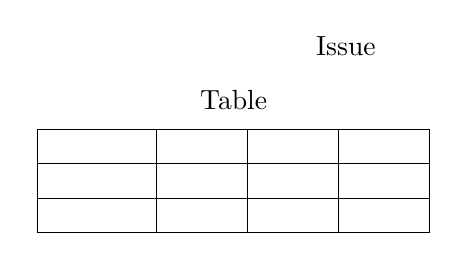
\begin{tikzpicture}[node distance=.8cm, remember picture]
				\node (issue_base) {};
				\node (issue_title) [right=of issue_base] {Issue};
				\node (issue_table) [below=of issue_base] {
					\begin{tabular}{|c|c|c|c|}
						\hline
						\hphantom{hello} \tikz \node (cell_anchor) {}; & \hphantom{hello} & \hphantom{hello} & \hphantom{hello} \\
						\hline & & & \\
						\hline & & & \\
						\hline
					\end{tabular}
				};
				\node at (issue_table.north) [anchor=south] {Table};
			\end{tikzpicture}
		};
		\node [below=of issue] (units) {
			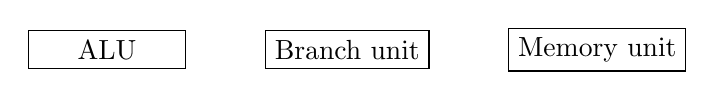
\begin{tikzpicture}[remember picture]
				\node[draw] [minimum width=2cm] (bu) {Branch unit};
				\node[draw] [minimum width=2cm, left=of bu] (alu) {ALU};
				\node[draw] [minimum width=2cm, right=of bu] (mu) {Memory unit};
			\end{tikzpicture}
		};
		\node[draw] [below=of units] (write_back) {Write back};
		\node[draw] [below=of write_back] (commit) {Commit};

		\node[draw] [right=of issue] (reorder_buffer) {
			
\begin{tikzpicture}
				\node {Reorder buffer};
			\end{tikzpicture}
		};

		\draw[->]  (fetch.north)        ++(0,1) -- node[right] {memory} (fetch.north);
		\draw[->]  (fetch.240)          -- node[left]  {instruction} (fetch.240|-decode.north);
		\draw[->]  (fetch.300)          -- node[right] {pc}          (fetch.300|-decode.north);
		\draw[->]  (decode.0)           -- ++(1,0) |- node[right, pos=0.25] {next pc} (fetch.15);
		\draw[->]  (decode.240)         -- node[left, align=center] {decoded\\instruction} (decode.240|-issue.north);
		\draw[->]  (decode.345)         -| node[right, align=center] {enqueue\\instruction} node[above right,pos=1] {\scriptsize +} (reorder_buffer);
		\draw[<->] (decode)             -- node[above] {rename} (register_file);
		\draw[<->] (issue)              -| node[left, align=center] {update\\available\\sources} (register_file);
		\draw[->]  (reorder_buffer)     |- node[right, align=center] {dequeue\\instruction} node[below right,pos=0] {-} (commit);
		\draw[->]  (issue_table.south)  |- ($(bu) +(0,0.5)$) node [left, pos=0.25, align=center] {take ready\\instruction} -- (bu.north) ;
		\draw[->]  (issue_table.south)  |- ($(alu)+(0,0.5)$) -- (alu.north);
		\draw[->]  (issue_table.south)  |- ($(mu) +(0,0.5)$) -- (mu.north) ;
		\draw[->]  (bu)                 -- ++(0,-0.5) -| node [right, pos=0.75] {result} (write_back);
		\draw[->]  (alu)                -- ++(0,-0.5) -| (write_back);
		\draw[->]  (mu)                 -- ++(0,-0.5) -| (write_back);
		\draw[->]  (write_back.175)     -| node[right, align=center, pos=0.65] {write\\result} ($(register_file.west)-(1,0)$) -- (register_file);
		\draw[->]  (write_back.185)     -| node[below, align=center, pos=0.25] {next pc} ($(fetch.west)-(6,0)$) -- (fetch);
		\draw[->]  (write_back)         -- node[left, align=center] {mark\\instruction done} (commit);

		\draw[->, dashed] (decode.15) -- ++(.5,0) |- node[pos=0.25,rotate=180,above,sloped] {block} (fetch.345);
		\draw[->, dashed] (issue.75) -- node[right] {block} (issue.75|-decode.south);
		\node (bu_anchor)  at ($(bu.east)+(.2,0)$) {};
		\node (alu_anchor) at ($(alu.east)+(.2,0)$) {};
		\node (mu_anchor)  at ($(mu.west)-(.2,0)$) {};
		\draw[->, dashed] (bu.east)  -- (bu_anchor)  -- node[left,pos=0.75] {block} (bu_anchor|-issue.south);
		\draw[->, dashed] (alu.east) -- (alu_anchor) -- node[left,pos=0.75] {block} (alu_anchor|-issue.south);
		\draw[->, dashed] (mu.west)  -- (mu_anchor)  -- node[right,pos=0.75] {block} (mu_anchor|-issue.south);

		\draw[->] (decode.240|-issue.north) -- ++(0,-0.5) -| (cell_anchor|-issue_table.north) -- ++(0,-0.15) node [above right] {\scriptsize +};

		\draw[thick] (current bounding box.south west) ++(-1,-1) rectangle ($(current bounding box.north east)+(1,1)$);
	\end{tikzpicture}
\end{center}
\end{document}